    
    % eventuell plot format noch anpassen, wie voce und RMSE plot sinnvoll einbauen?
    % sind RMSE plots überhaupt notwendig bei validation?
    % strain-strain plot bei verification einfügen
    
    \chapter{Results}

    In this chapter the results from different test cases presented in section XX will be evaluated. First, we discuss the verification results to understand the general behavior of the optimization process. In the next step we validate the optimization performance using different data sets. 
    Finally, we present the results of the cyclic load cases.

    
    \section{Verification}\label{verification}

    In this section, we discuss the results of the data set used for the verification of our optimization process. To evaluate the quality of the optimization process, we define characteristic quantities and investigate their evolution. 
    Noch den load case kurz aufschreiben.


    \begin{figure}[H]
		\centering
        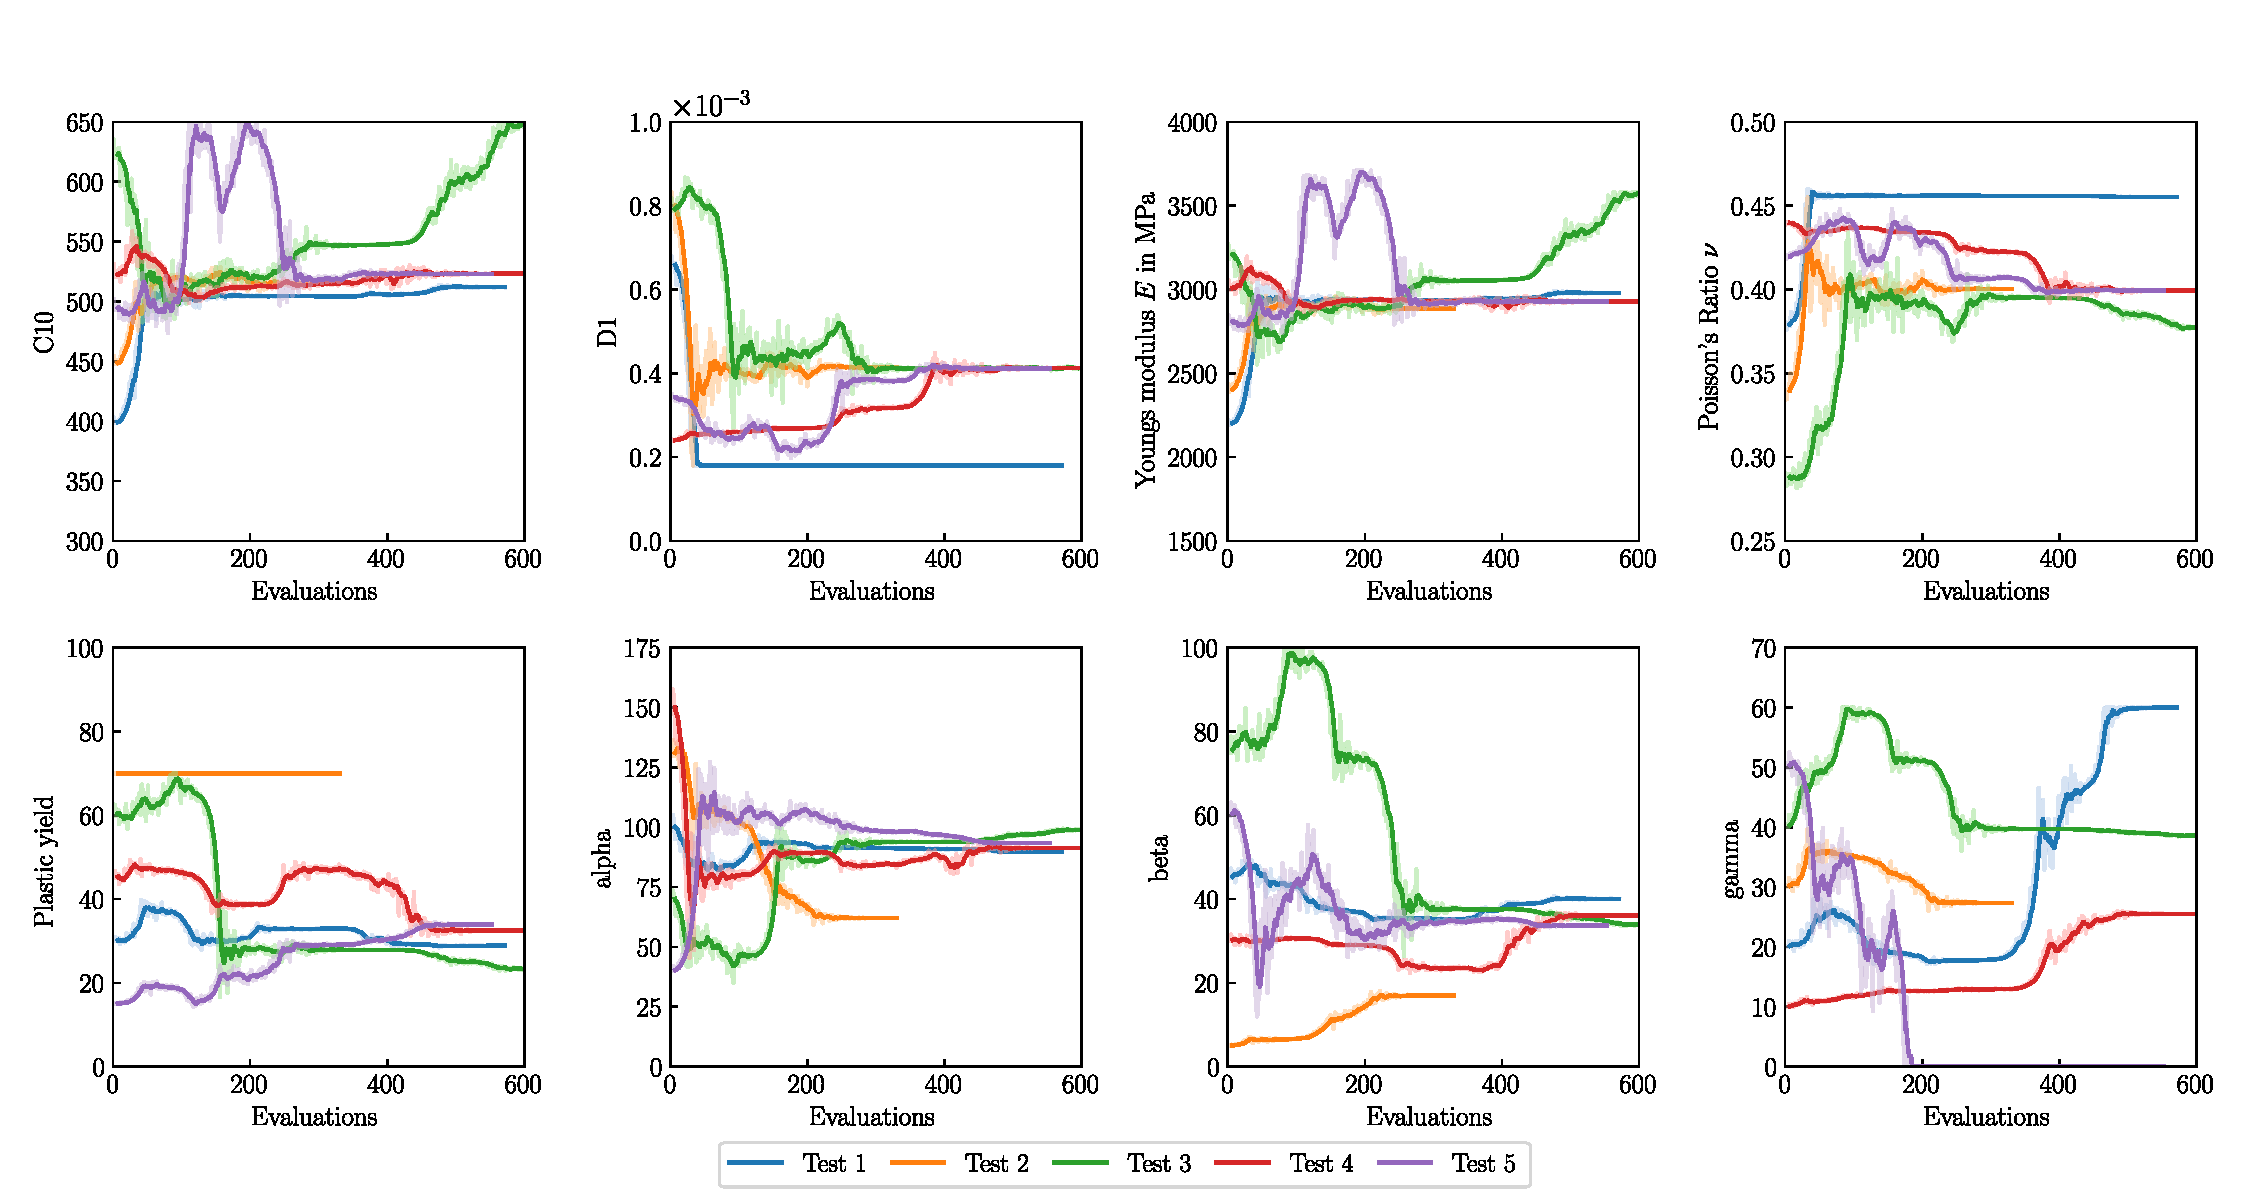
\includegraphics[width=0.7\textwidth]{verify_material_params.pdf}
		\caption{optimization progress of material parameters}
		\label{fig:materialparameters}
	\end{figure}
    As process quantities we log the evolution of the material parameters during the optimization. Since these are our input parameters we performed multiple tests with varying parameter combinations to evaluate the stability of our program. The results are presented in \ref{fig:materialparameters}. In the first row the elastic material parameters are presented. For a better understanding, we transformed the hyper-elastic parameters \(C10\) and \(D1\) into Young's modulus \(E\) and Poisson ratio \(\nu\). In the second row the plastic material parameters are presented. For elastic and plastic parameters we can observe convergence for every parameter combination. However, the converged solutions differ from each other for most of the combinations. 
    For a detailed discussion of possible reasons we separate between elastic and plastic material behavior. Since our tested material shows an elastic response only up to the second data point, there might be not enough optimization points to find an unique solution for the elastic material parameters. Nevertheless, we have to investigate other characteristic quantities to ensure our assumption and understand the influence of the plastic parameters. In \autoref{fig:progress stress-strain curve} the progress of the stress-strain curve in normal direction during one exemplary test together with the target curve from the MD simulation is presented. The optimized curve matches the target curve after only  \(25 \%\) of the evaluations. Since the stress-strain curve is one of our target data this progress indicates a correct optimization behavior of our algorithm. To support this assumption the final stress-strain curves of the test series are depicted in \autoref{fig:final stress-strain curves}. Despite the high variance of the final material parameters, the stress-strain curves all matches the target data for the stress-strain curve in normal direction. Because of this deviation we depicted the influence of the parameters on the trend of the VOCE-hardening curve shown in \autoref{fig:Parameter influence on VOCE-hardening curve}. The parameter alpha has the greatest impact on the shape of the curve, while a variety of \(50\%\) in the parameter gamma has hardly any visible effect. This leads to a high flexibility in adjusting the shape of the curve and as a consequence to multiple possible parameter combinations to fit the target curve. To support our assumption we check the quality of the optimization result by plotting the progress of the root mean squared error (RSME) for all the tests in \autoref{fig:rmse progress}. We observe that a common minimum RMSE value is reached in all optimization runs, indicating that the results are of equivalent quality. 
    The results of this verification tests lead to some states about the quality of the optimization algorithm. The results of the stress-strain data show a good match of the optimized curve with the target data for every test which is confirmed by the RMSE. In contrast we observe a high variance in final the material parameters found by the algorithm. These results suggest that the algorithm can generally find parameter values to match the target data. However, the variance in these optimal parameters shows that multiple parameter combinations lead to the same quality of result. This behavior may be due to the relatively large number of optimization parameters compared to the dimension of the target data. To verify this assumption we reduced the number of material parameters. Since only the first point of the target data lies in the elastic domain, we fixed the elastic material behavior and computed them directly from the data of the first point. Then we tested this new configuration of the algorithm with the current target data and two other data sets.


    \begin{figure}[H]
        \centering
        \subfigure[evolution of stress-strain curve]{
            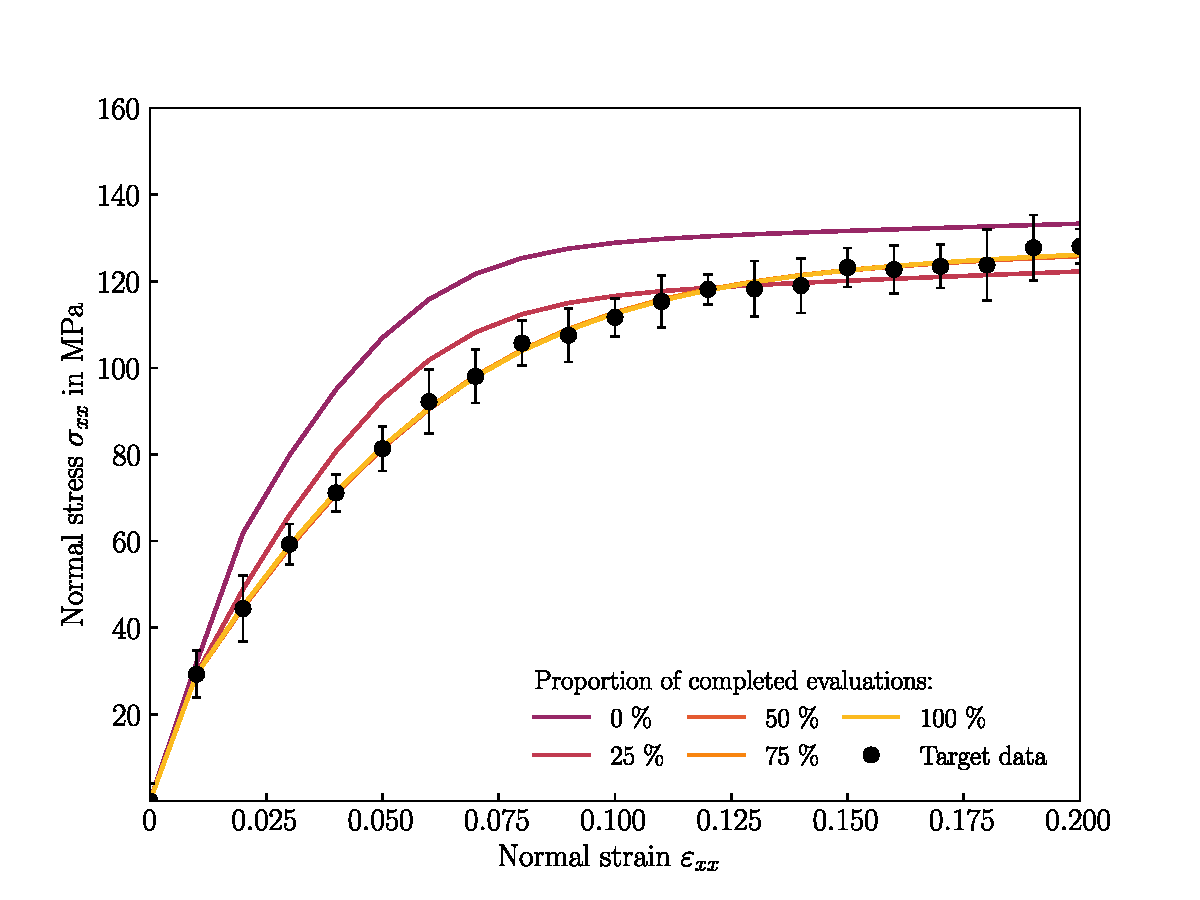
\includegraphics[width=0.47\textwidth]{verfiy_stress_strain_progress.pdf}
            \label{fig:progress stress-strain curve}
        }
        \subfigure[final stress-strain curves]{     
            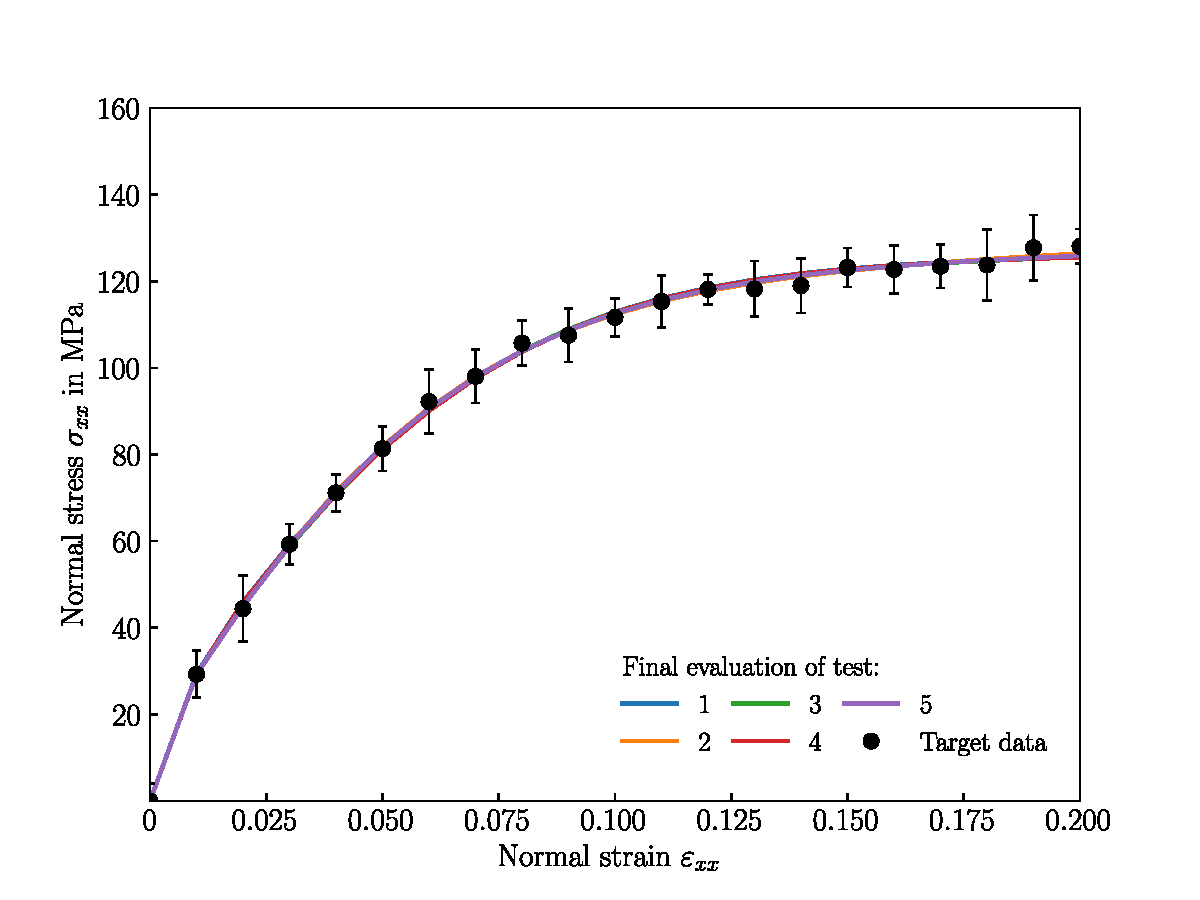
\includegraphics[width=0.47\textwidth]{verify_stress_strain_combined.pdf}
            \label{fig:final stress-strain curves}
        }
        \caption{a) evolution of the stress-strain curves during optimization for exemplary test, b) final stress-strain curves for complete test study}
        \label{fig:complete}
    \end{figure}


   
   \begin{figure}
		\centering
        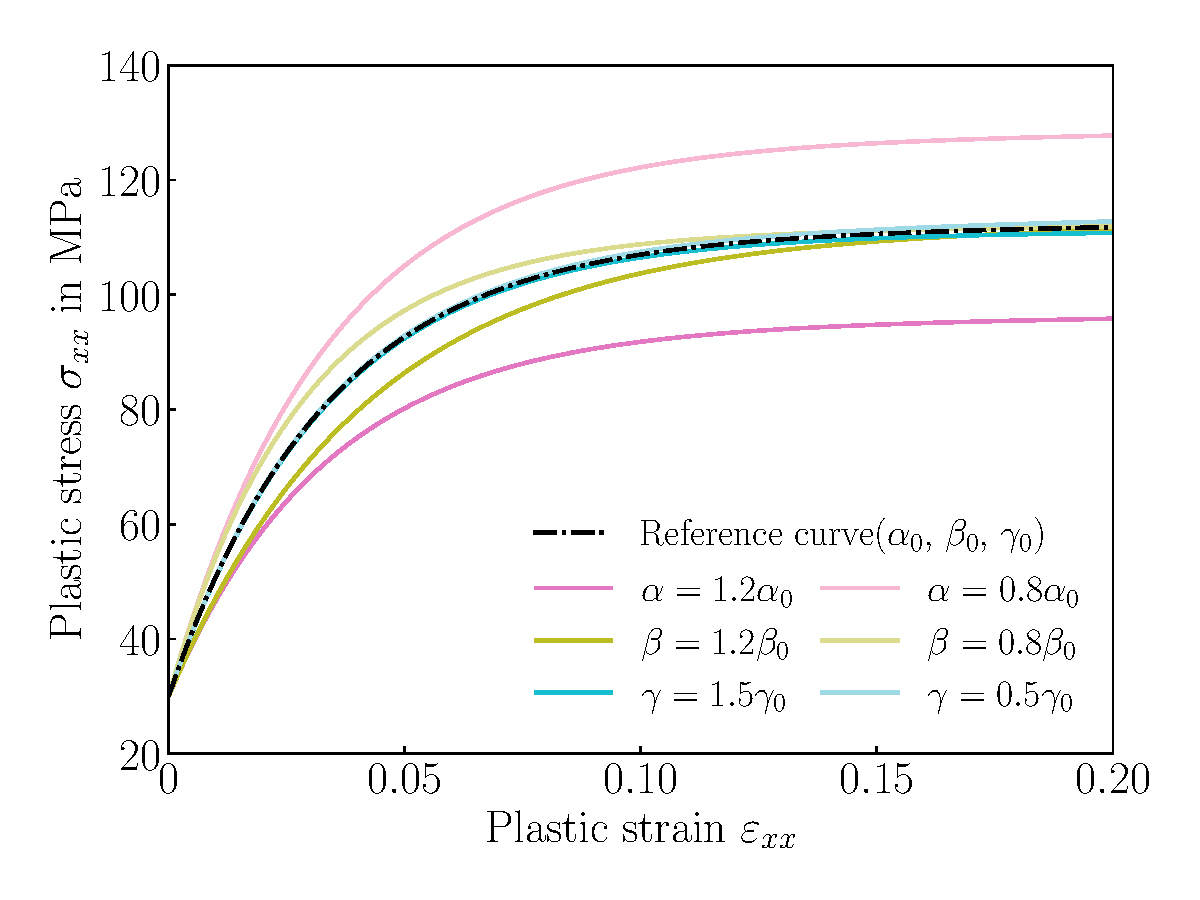
\includegraphics[width=0.5\textwidth]{voce_curve.pdf}
		\caption{parameter influence on voce-hardening curve}
		\label{fig:Parameter influence on VOCE-hardening curve}
	\end{figure}
    PICTURES with Krümmung und Steigung --> parameters to characterize curve

    \begin{figure}[H]
		\centering
        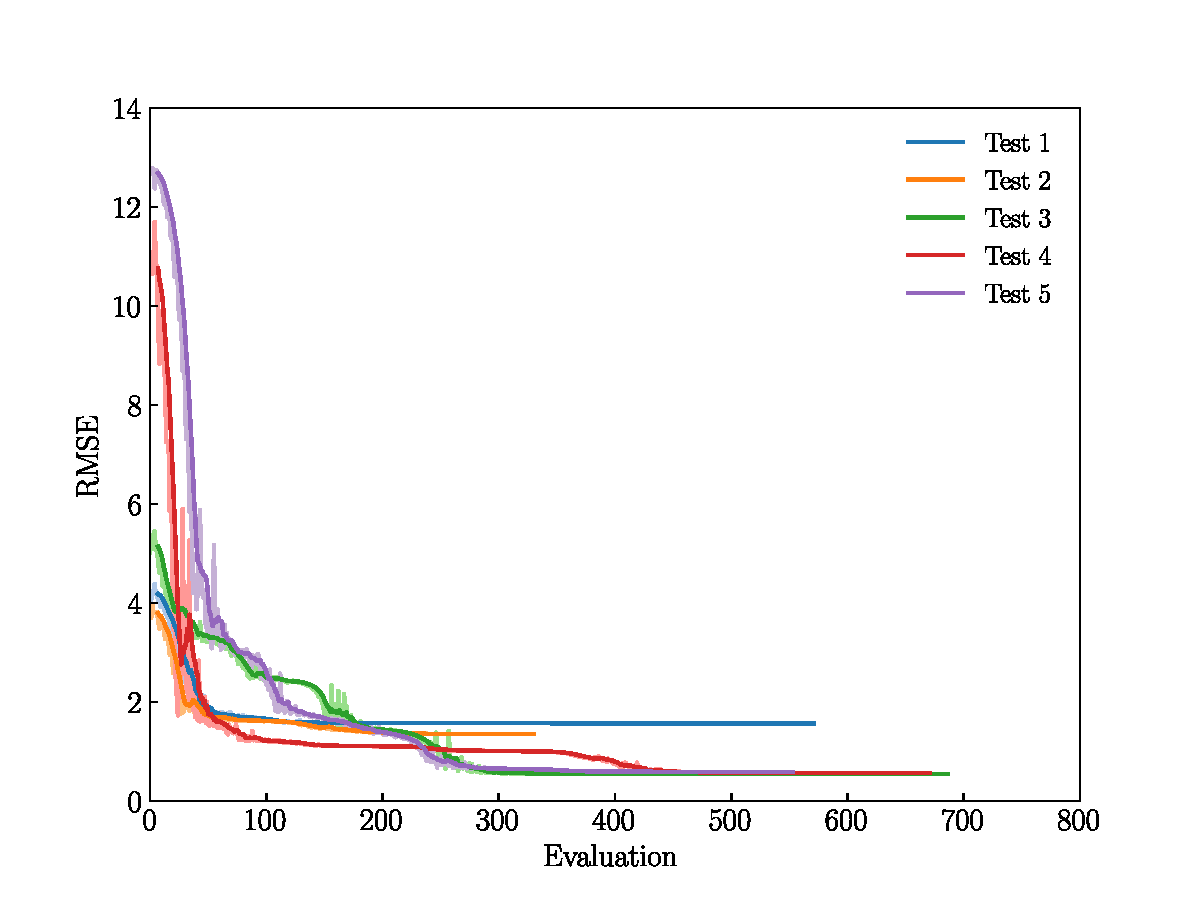
\includegraphics[width = 0.7\textwidth]{verify_rsme.pdf}
		\caption{rmse for multiple tests}
		\label{fig:rmse progress}
	\end{figure}

    
    \section{Validation}
    To improve our algorithm we reduced the number of optimization parameters by fixing the elastic material parameters. The results of this implementation for three different data sets will be discussed in this section.

    \begin{figure}[H]
		\centering
        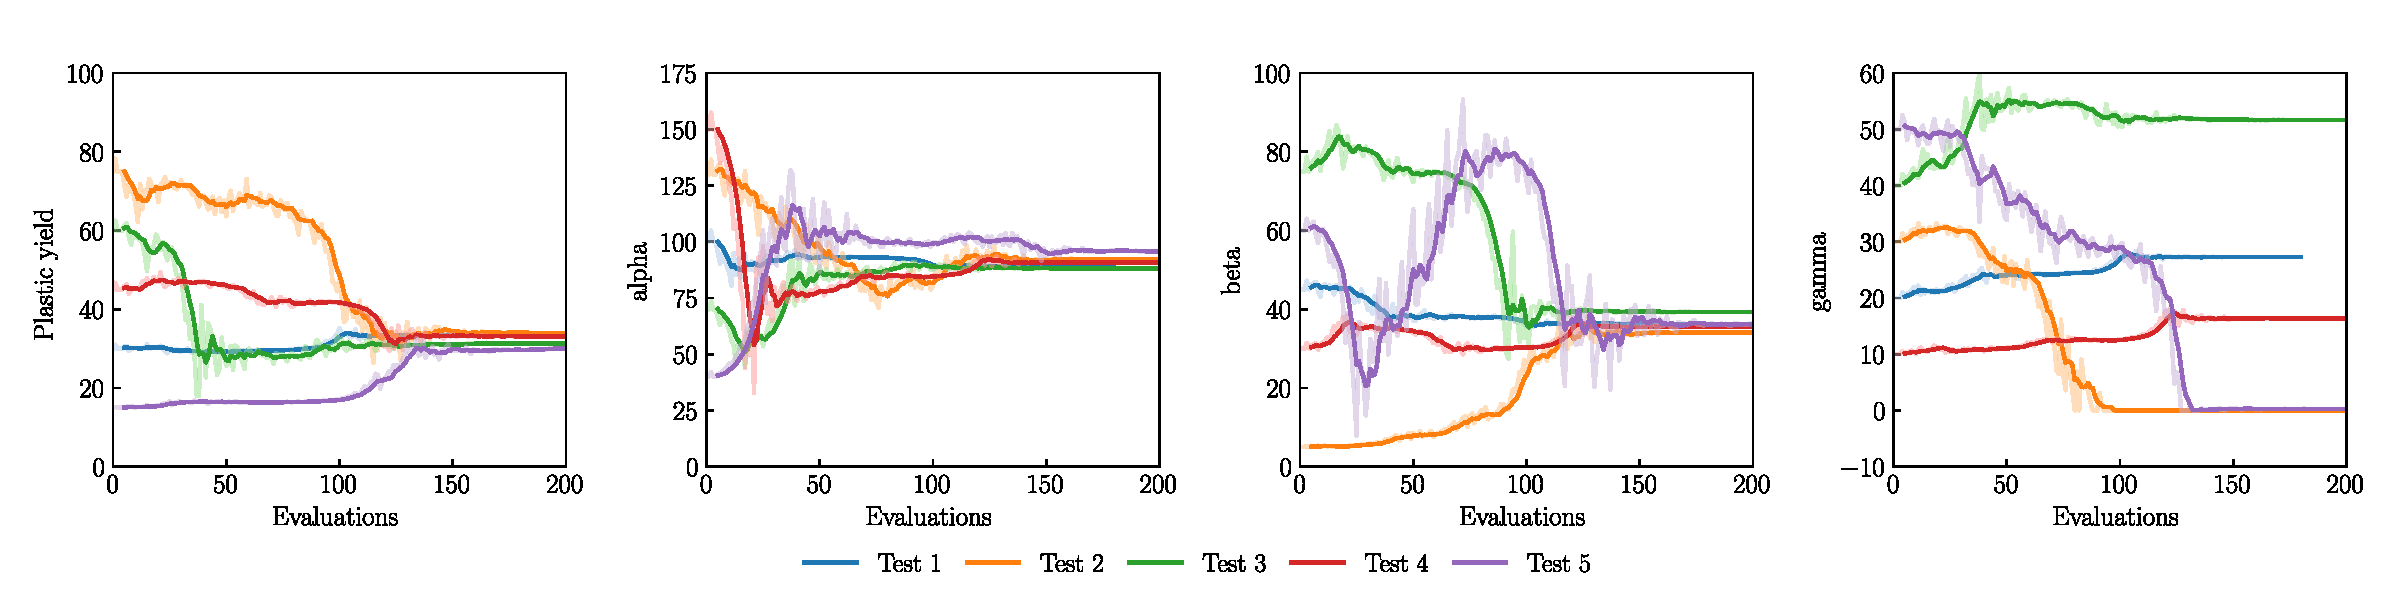
\includegraphics[width=0.47\textwidth]{valid6to3_material_params.pdf}
		\caption{progress of material parameters for validation tests}
		\label{fig:validation material params 6to3}
	\end{figure}

    In the first step we used the same data set as in \autoref{verification} to test the modified algorithm. The optimized plastic material parameters are shown in \autoref{fig:validation material params 6to3}.  In all tests, the values of the plastic yield, alpha and beta demonstrate a converging trend towards a singular solution. The only exception to this is gamma whose converged values vary for each individual test. As was outlined in the preceding discussion, gamma exerts minimal influence on the trend of the hardening curve. Consequently, the focus shall be directed towards the plastic yield, alpha and beta, which indicate an improvement in their optimization behavior.
    The quality of this optimized parameters is ensured through the match of the stress-strain curves with the target data. As demonstrated in \autoref{fig:validationStressStrain6to3} the final stress-strain curves exhibit a strong correlation with the target data. The evolution of the RMSE XXX supports this results with small values for every test. A comparison of the results of the present study with those of the verification study reveals an equivalent level of optimization quality. Additionally, the results of the material parameters indicate a positive impact of the algorithm modification, showing a unique solution for the important parameters. 
     
    
    \begin{figure}
        \centering
        \begin{minipage}[t]{0.47\textwidth}
            \centering
            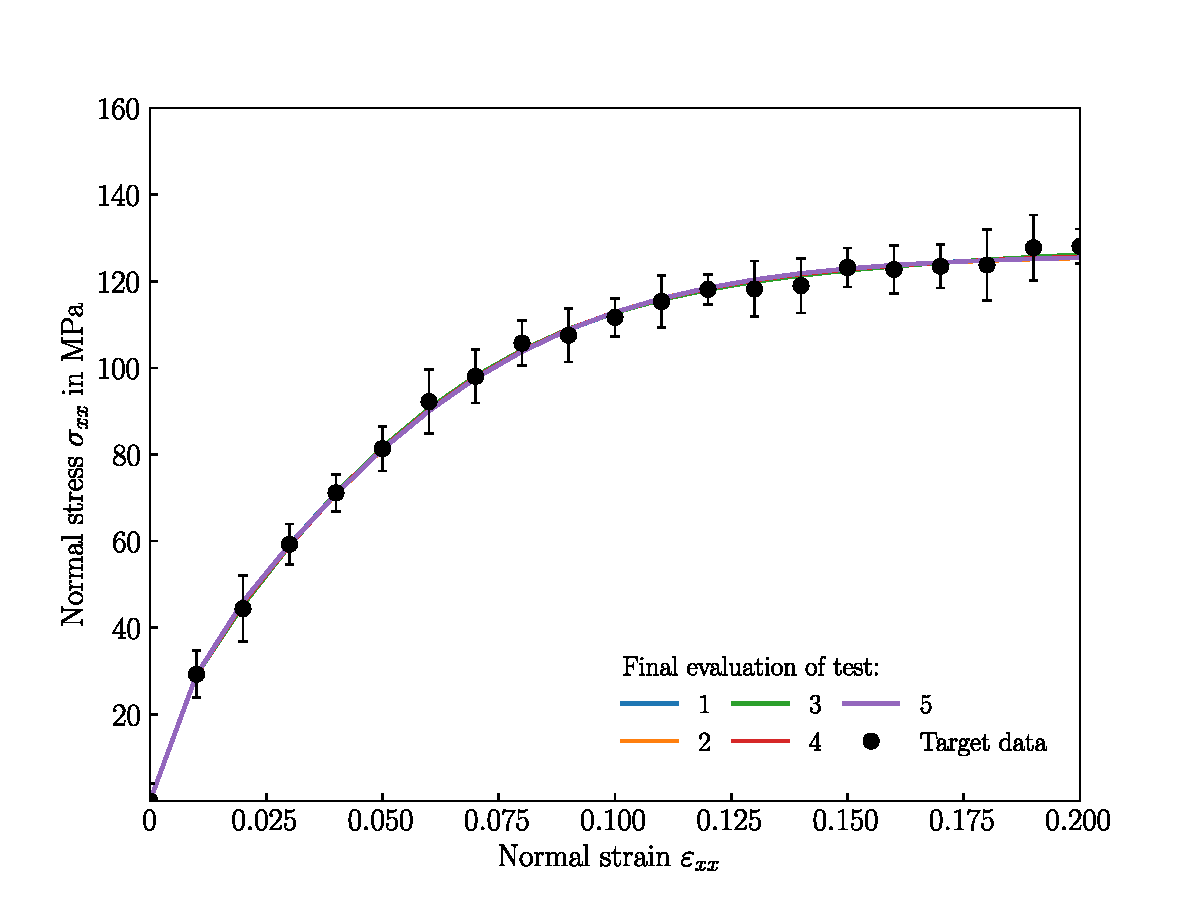
\includegraphics[width=\textwidth]{valid6to3_stress_strain_combined.pdf}
            \caption*{(a) Final stress-strain curves}
            \label{fig:validationStressStrain6to3}
        \end{minipage}
        \hfill
        \begin{minipage}[t]{0.47\textwidth}
            \centering
            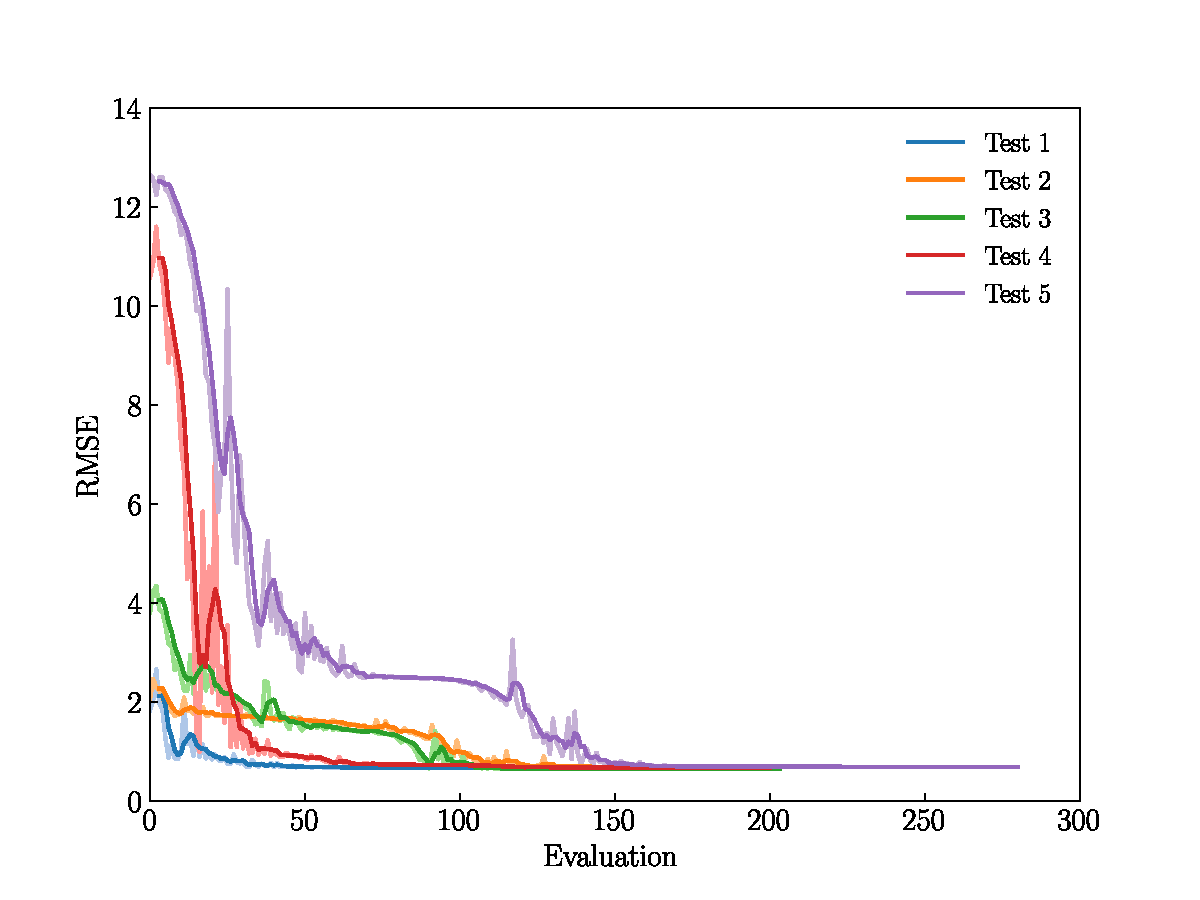
\includegraphics[width=\textwidth]{valid6to3_rsme.pdf}
            \caption*{(b) RMSE evolution}
            \label{subfigure:validation-rmse-6to3}
        \end{minipage}
        \caption{Results of validation tests with 6to3 dataset}
        \label{fig:validation results 6to3}
    \end{figure}
    


    To verify our algorithm independent of the used target data set, we made the same tests with two additional data sets. In the following we present the results of studies for mixing ratio 4:3 and 8:3. 

    \begin{figure}[H]
        \centering
        \subfigure[evolution of material 4:3]{
            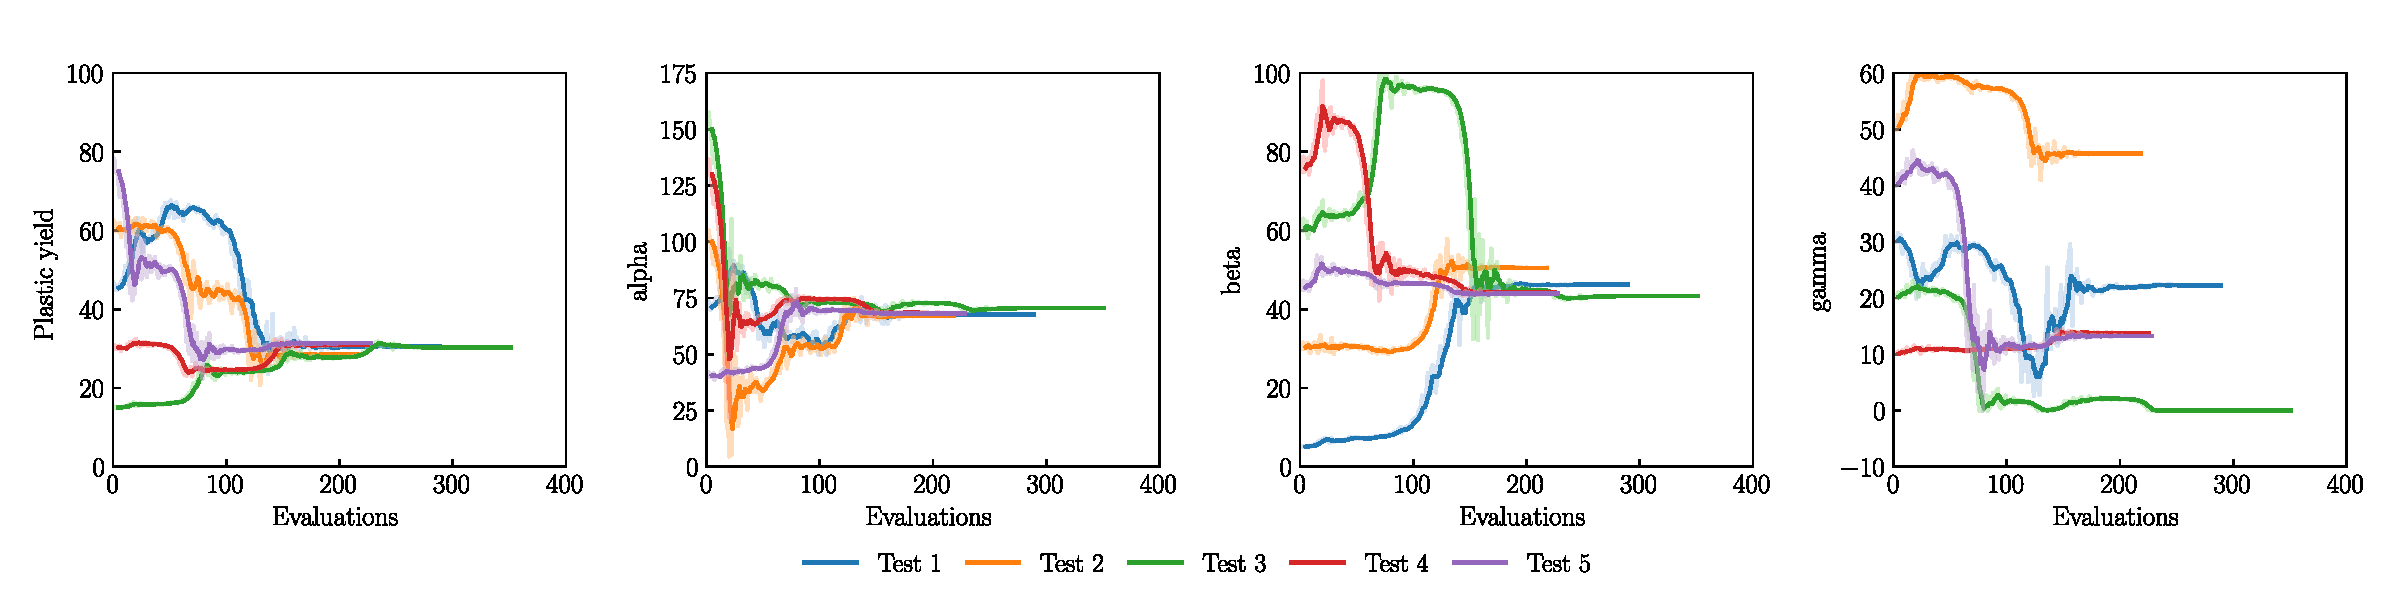
\includegraphics[width=1.0\textwidth]{valid4to3_material_params.pdf}
    		\label{fig:material params 4to3}
        }
        \subfigure[evolution of 8:4]{
            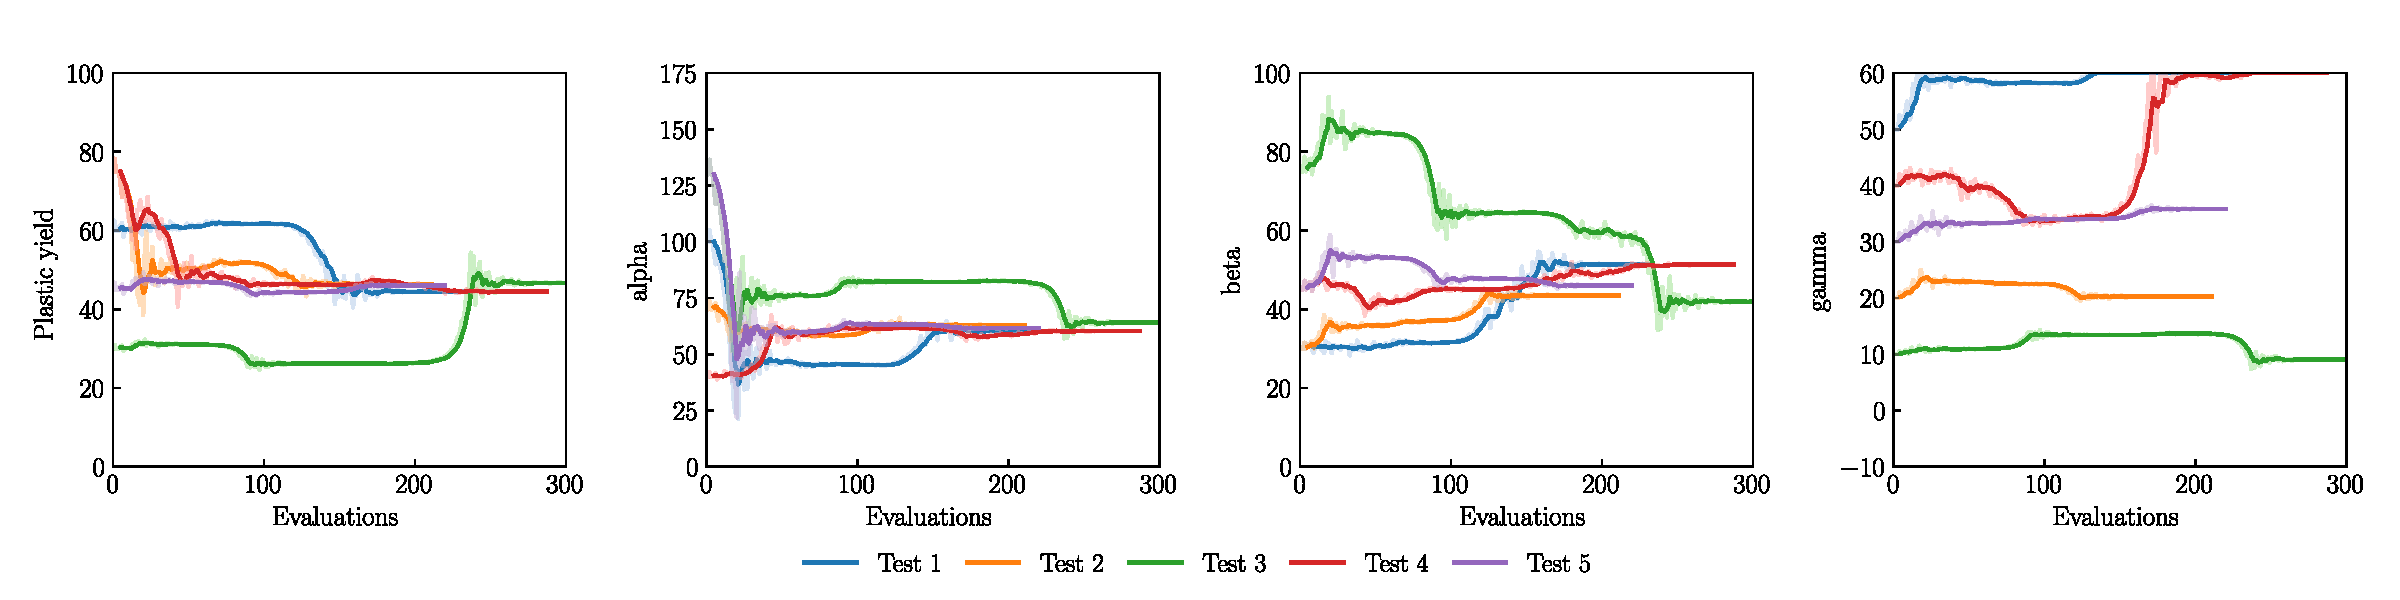
\includegraphics[width=1.0\textwidth]{valid8to3_material_paramspdf.pdf}
            \label{fig:material params 8to3}
        }
        \caption{Evolution of material parameters for a) mixing ratio 4:3 and b) mixing ratio 8:3}
        \label{fig:validation material params}
    \end{figure}

    The evolution of the plastic material parameters for the mixing ratios 4:3 and 8:3 in plotted in \autoref{fig:validation material params}. We can observe a similar convergence behaviour as in the validation study with mixing ratio 6:3. Only test case 3 for mixing ratio 8:3 shows a deviation provided that all values converge quite late. Since we chose the initial values randomly this might occur through an unfavourable combination of values. 
    In \autoref{fig:validation results} we represent the optimized stress-strain curves and the evolution of the RMSE. For all tests the stress-strain values correlate with the target data. The equivalent level of the RMSE for the converged solutions indicate a similar quality of the optimization result for all tests. These results indicate an improvement of the solution results through determining the elastic parameters.
     
    \begin{figure}[H]
        \centering
        \subfigure[stress-strain curves]{
            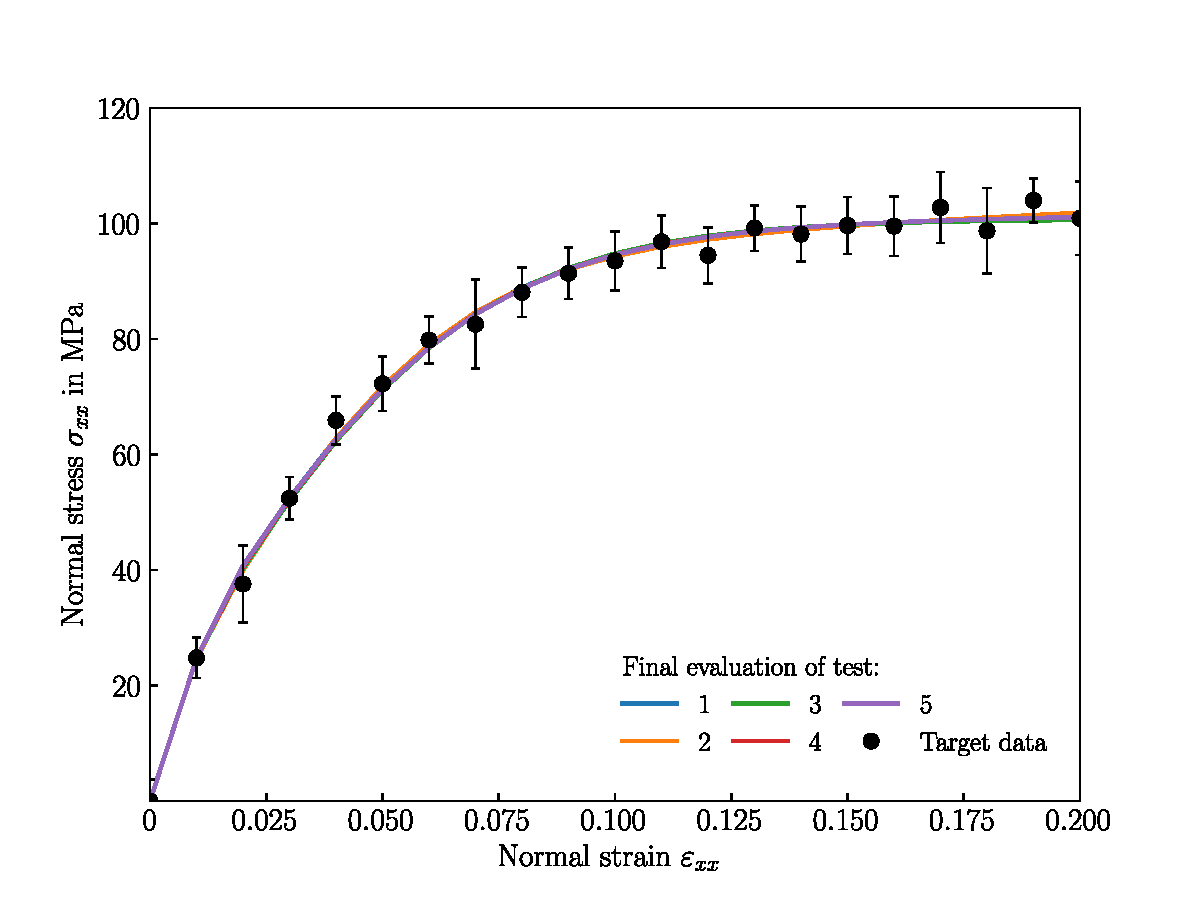
\includegraphics[width=0.47\textwidth]{valid4to3_stress_strain_combined.pdf}
    		\label{fig:validation stress-strain curves 4to3}
        }
        \subfigure[RMSE evolution]{
            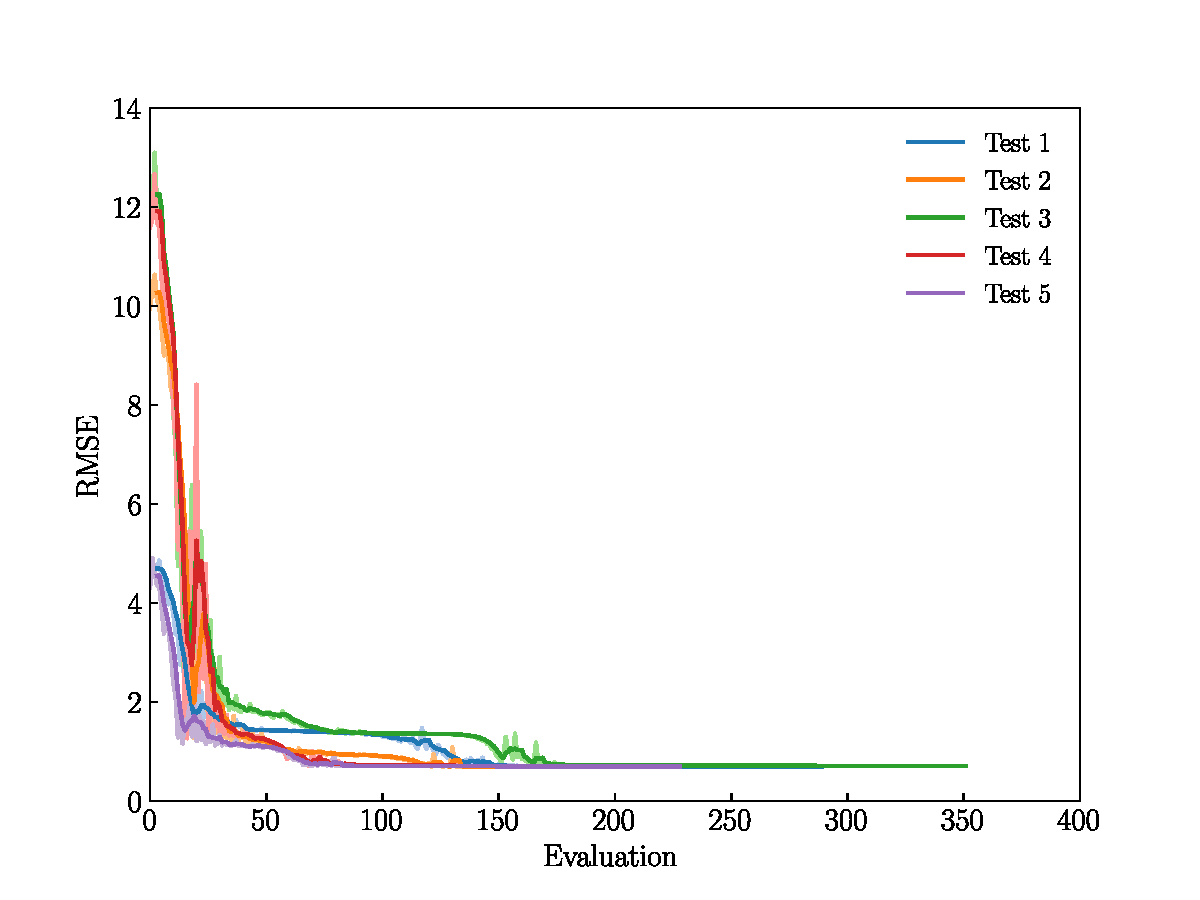
\includegraphics[width=0.47\textwidth]{valid4to3_rmse.pdf}
            \label{fig:validation rmse 4to3}
        }
        \subfigure[Final stress-strain curves]{
            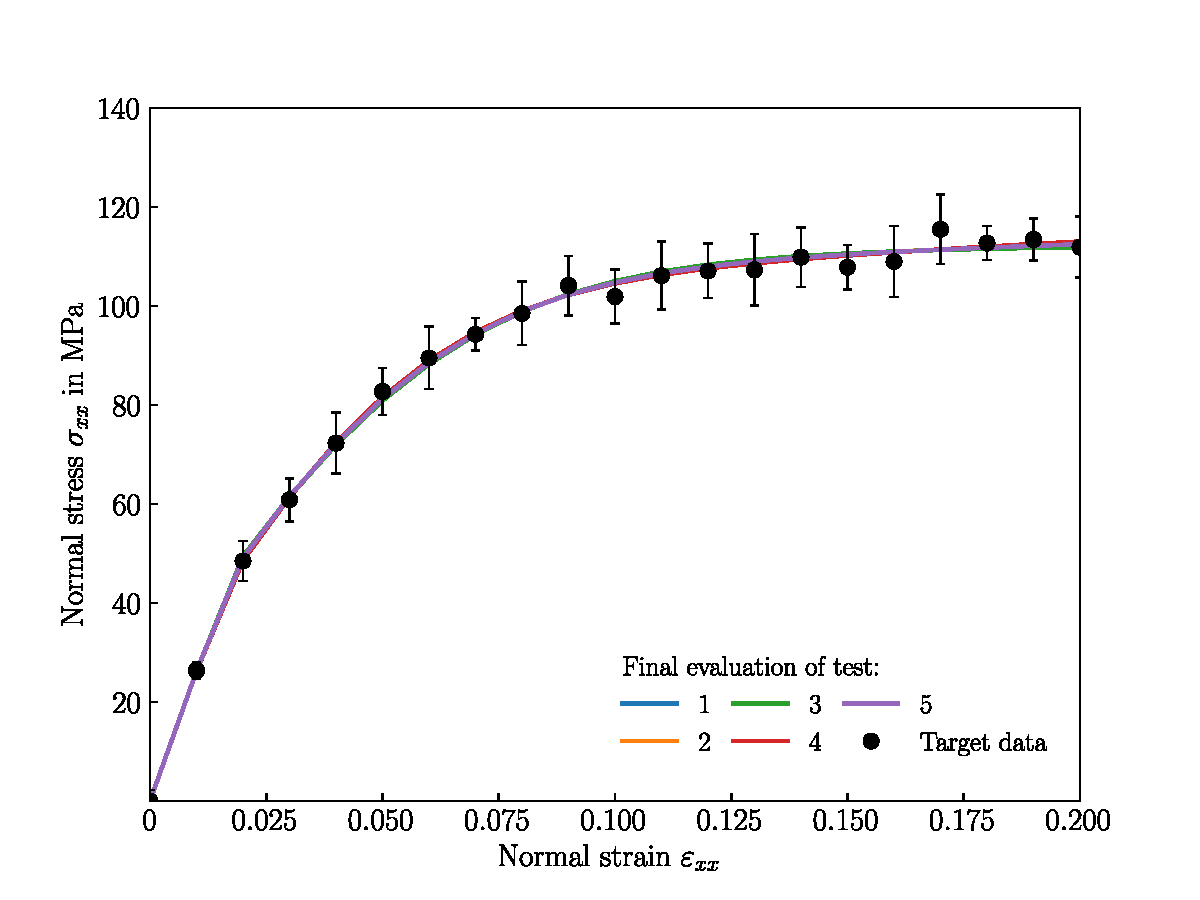
\includegraphics[width=0.47\textwidth]{valid8to3_stress_strain_combined.pdf}
    		\label{fig:validation stress-strain curves 8to3}
        }
        \subfigure[RMSE evolution]{
            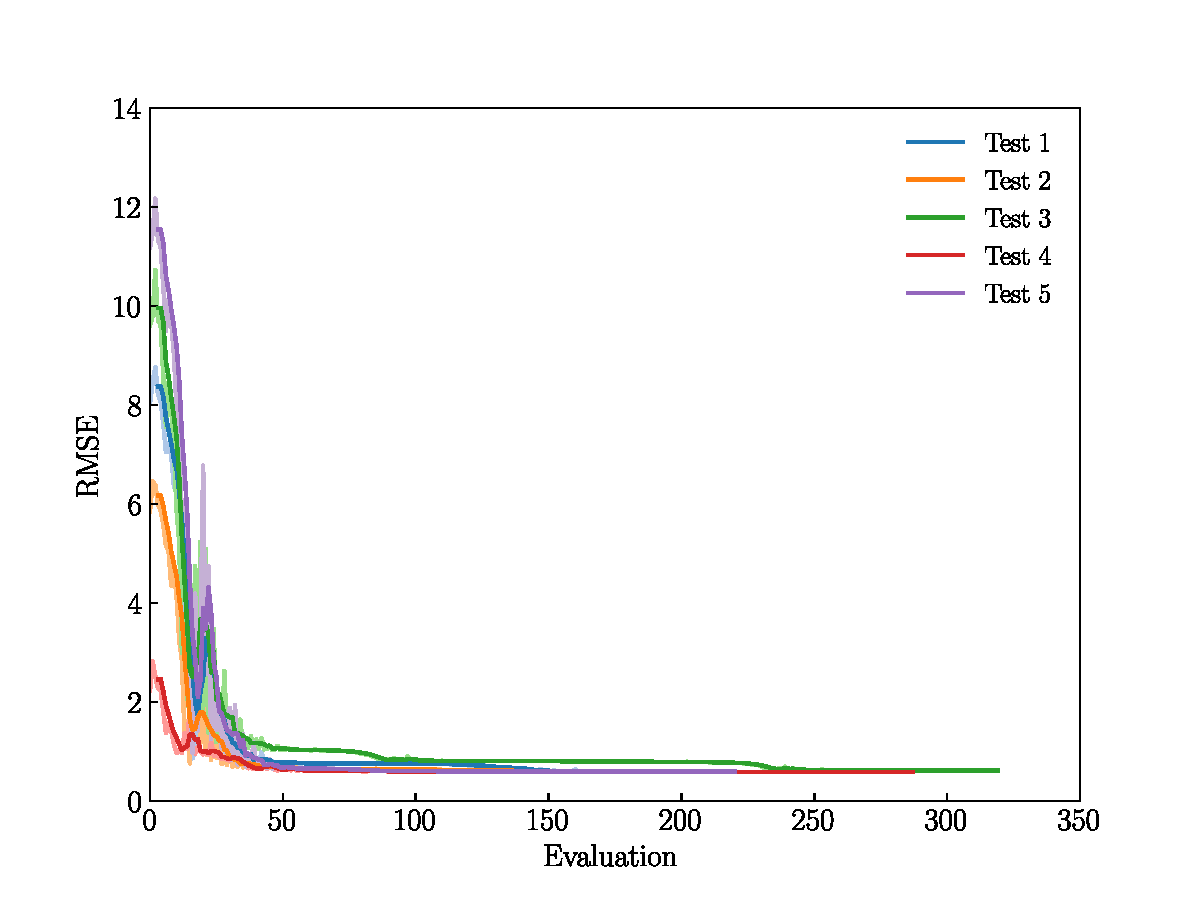
\includegraphics[width=0.47\textwidth]{valid8to3_rmse.pdf}
            \label{fig:validation rmse 8to3}
        }
        \caption{Results of validation tests with mixing ratios 4:3 and 8:3: a) final stress-strain curves for mixing ratio 4:3, b) RMSE for mixing ratio 8:3, c) final stress-strain curves for mixing ratio 4:3, d) RMSE for mixing ratio 8:3}
        \label{fig:validation results}
    \end{figure}

    Overall these results demonstrate the reliability of the optimization algorithm for the load case of a single tensile strain in one direction with fixed elastic parameters. The specification of the elastic parameter values improves the optimization performance in a way that for the plastic yield, alpha and beta independent of the initial values a singular solution can be found. However, the manual specification of Youngs modulus and Poisson ratio is only possible for target data sets with exactly one data point in the elastic domain of the material. For data sets with multiple points in the elastic domain a manual specification becomes complicated quite fast. Additional, for materials with completely unknown material behaviour, the point of transition between elastic and plastic behaviour is still unknown. In order to process such data sets too, we need to integrate the elastic parameters in the optimization process. In doing so the singularity of the solution should be maintained. Therefore the algorithm needs additional information about the mechanical material behaviour. In the following step we tried to do so through the combination of two load cases. Additional to the already tested tensile strain we applied a shear strain. As described in section XX the shear modulus contains information about Youngs modulus and  Poisson ratio what might improve the performance of the optimizatoin process. The information contained within the shear modulus about Youngs modulus and Poisson ratio might enclose the necessary restrictions to reduce the solution variability. 
    
    Warum sinusförmige belastung? Jz schon mit zyklischen versuchen kommen?
    

    \section{shear and normal strain tests combined}
    \section{cyclic tests}







	